\documentclass{article}

\usepackage[LGR, T1]{fontenc}
\usepackage[utf8]{inputenc}
\usepackage[greek,english]{babel}
\usepackage{alphabeta}
\usepackage{graphicx}
\usepackage{verbatim}
\usepackage{float}

\graphicspath{{./}}


\author{Στεφανίδης Ιωάννης}
\title{Δίκτυα Υπολογιστών ΙΙ}
\date{ΑΕΜ: 9587}


\begin{document}

\maketitle

\center
{\huge{Wireshark}}

\section{Echo}
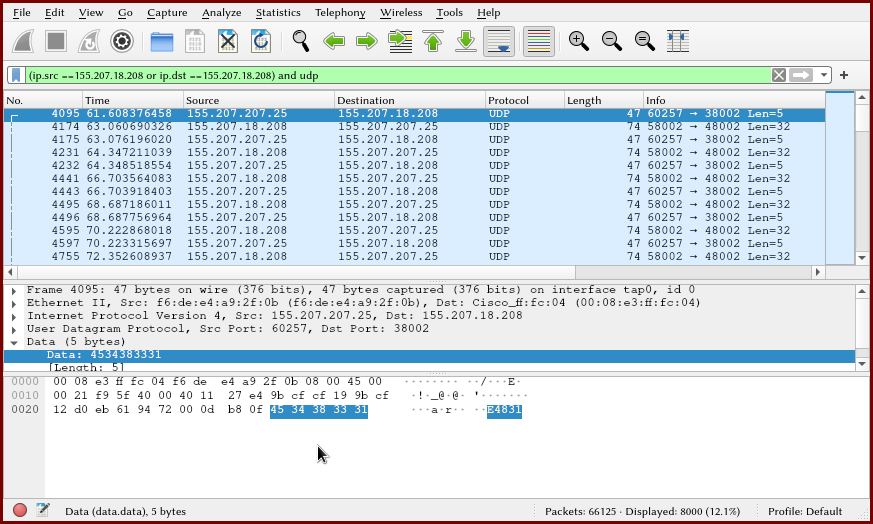
\includegraphics[width=\textwidth]{wireshark1.png}
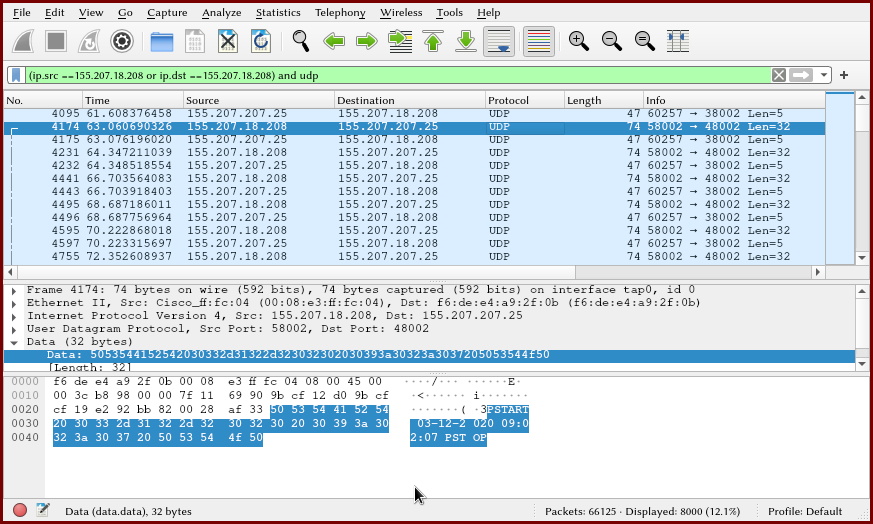
\includegraphics[width=\textwidth]{wireshark2.png}

\section{Image}
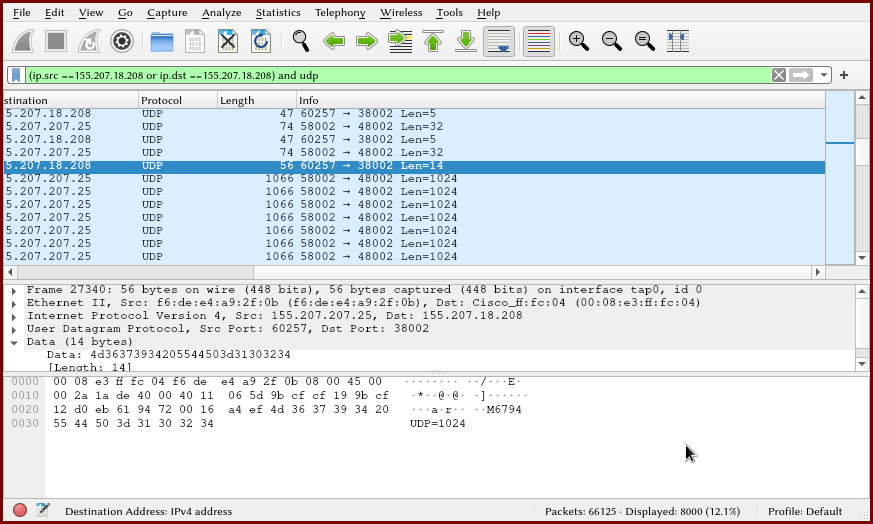
\includegraphics[width=\textwidth]{wireshark3.png}
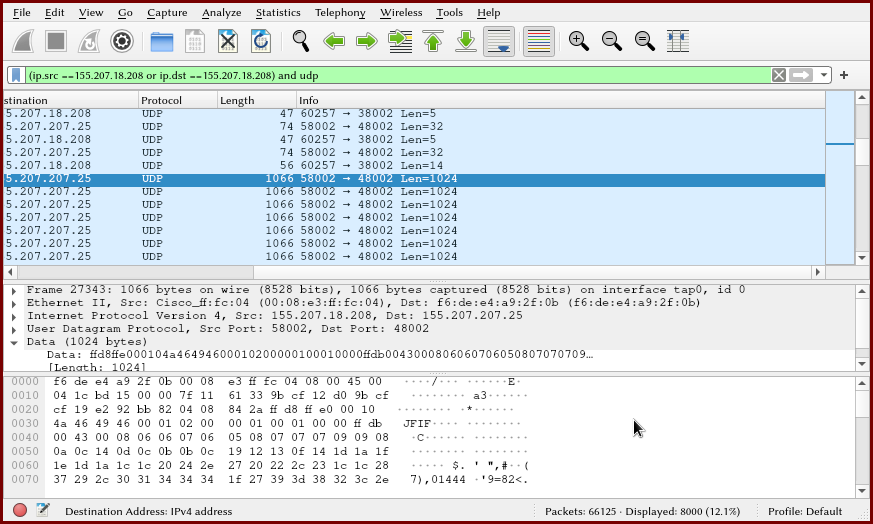
\includegraphics[width=\textwidth]{wireshark4.png}
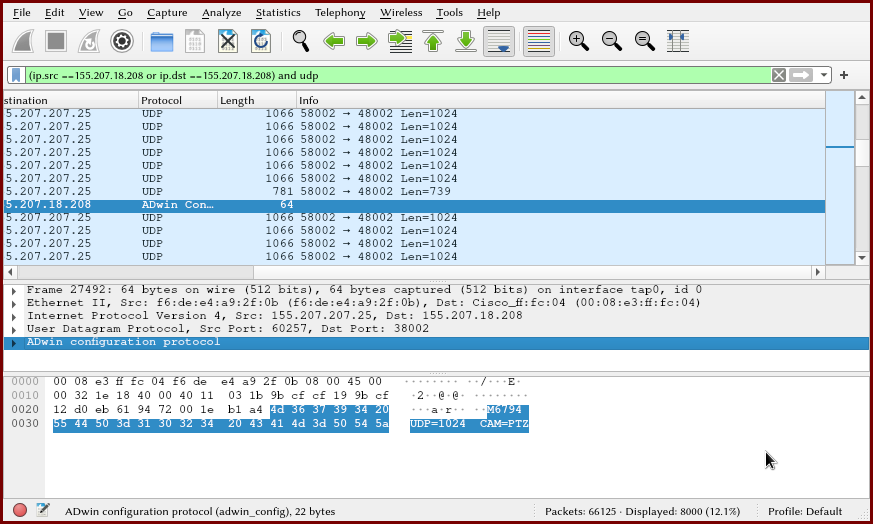
\includegraphics[width=\textwidth]{wireshark5.png}
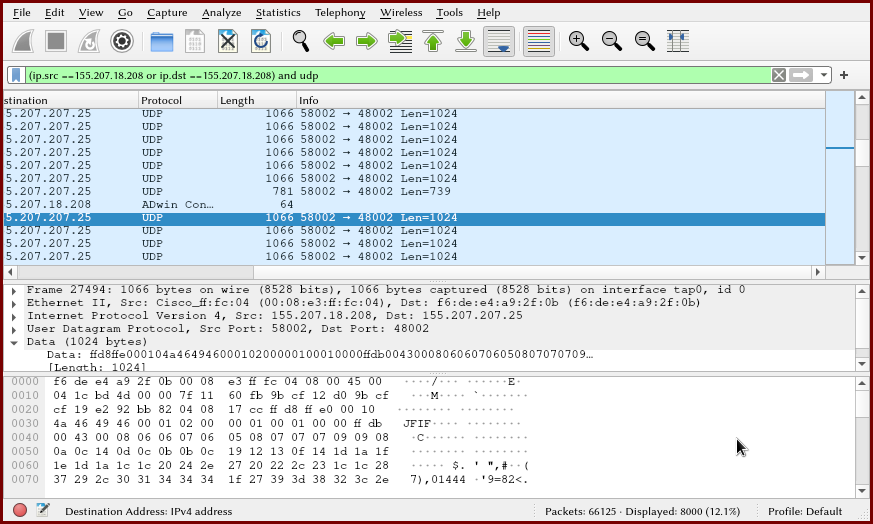
\includegraphics[width=\textwidth]{wireshark6.png}

\section{Temperatures}
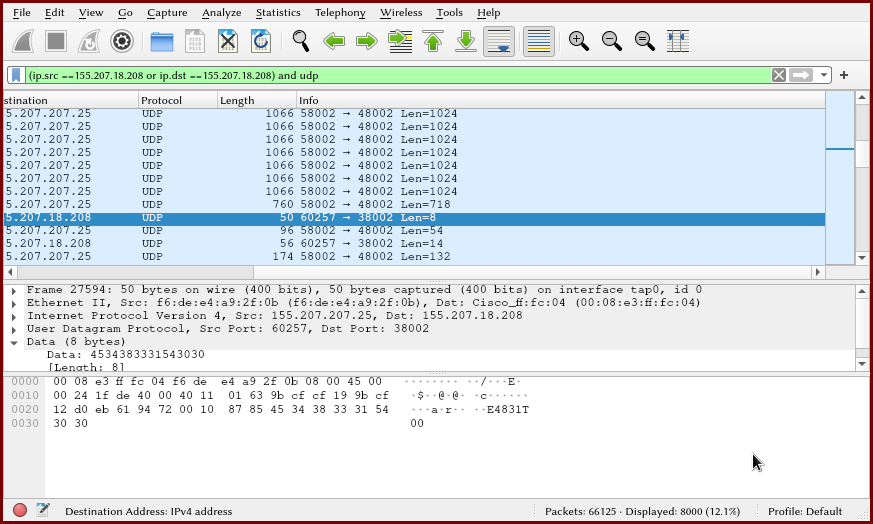
\includegraphics[width=\textwidth]{wireshark7.png}
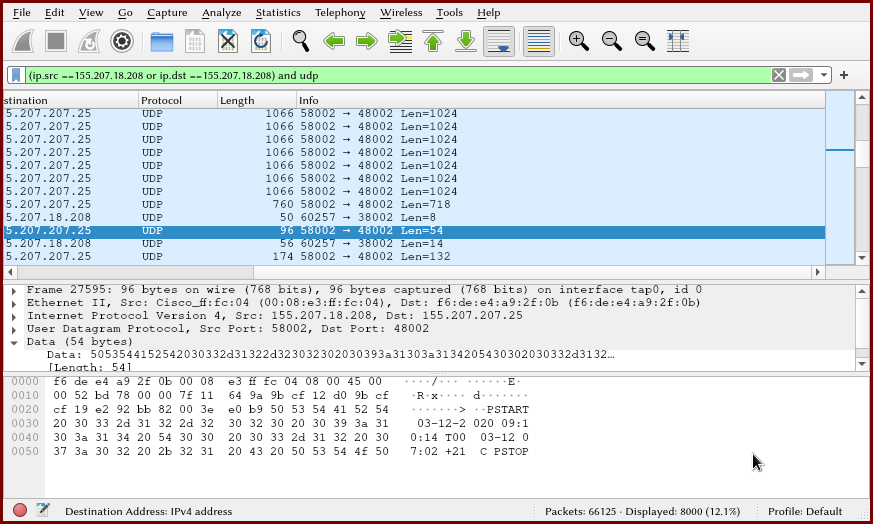
\includegraphics[width=\textwidth]{wireshark8.png}

\newpage
\section{Sound}

Κατά την εκτέλεση της εφαρμογής μου κατέβασα 2 φορές το τραγούδι 01
και μετά έτρεξα ξεχωριστά το πρόγραμμα μόνο για το τραγούδι 02 το οποίο
ξέχασα να καταγράψω.

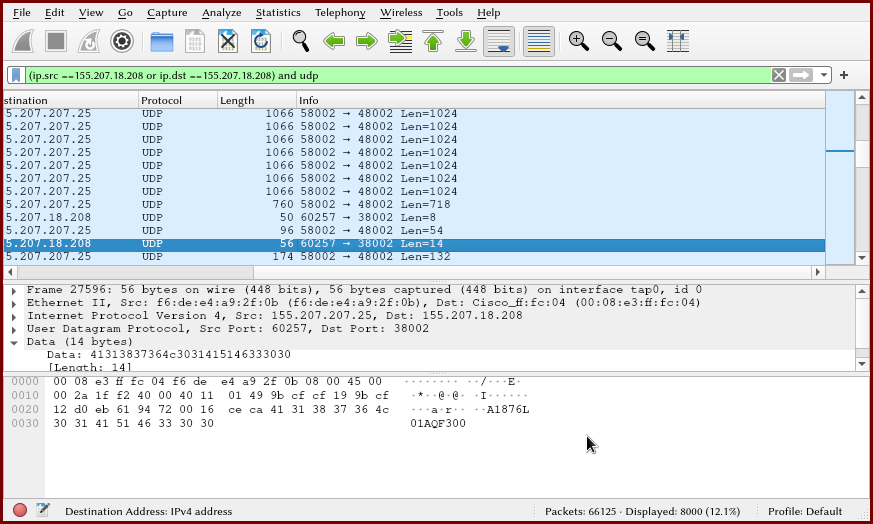
\includegraphics[width=\textwidth]{wireshark9.png}
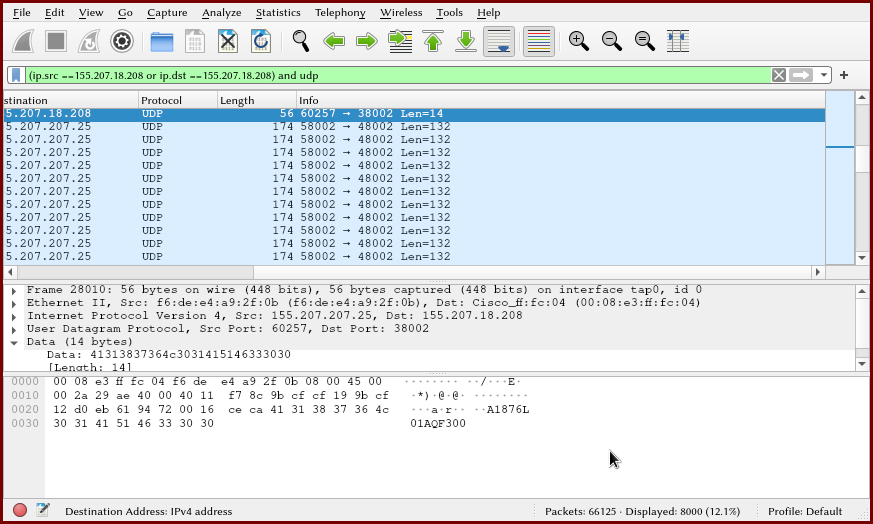
\includegraphics[width=\textwidth]{wireshark10.png}
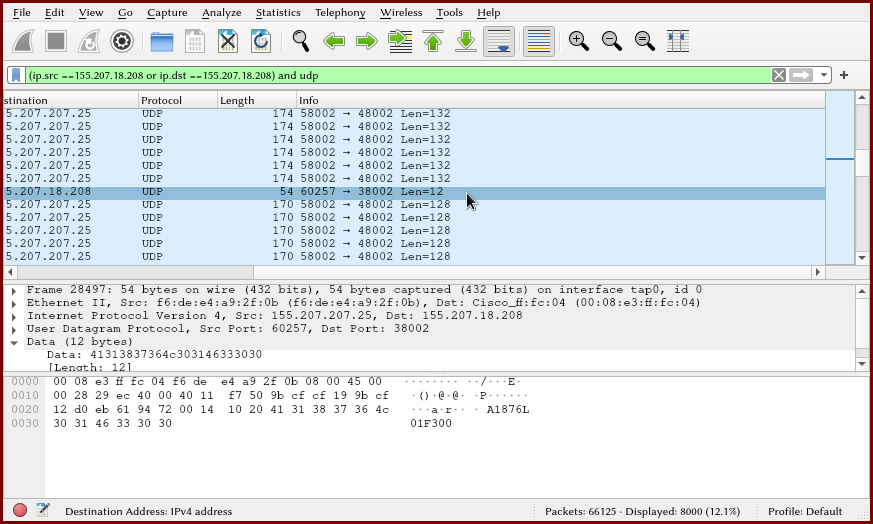
\includegraphics[width=\textwidth]{wireshark11.png}
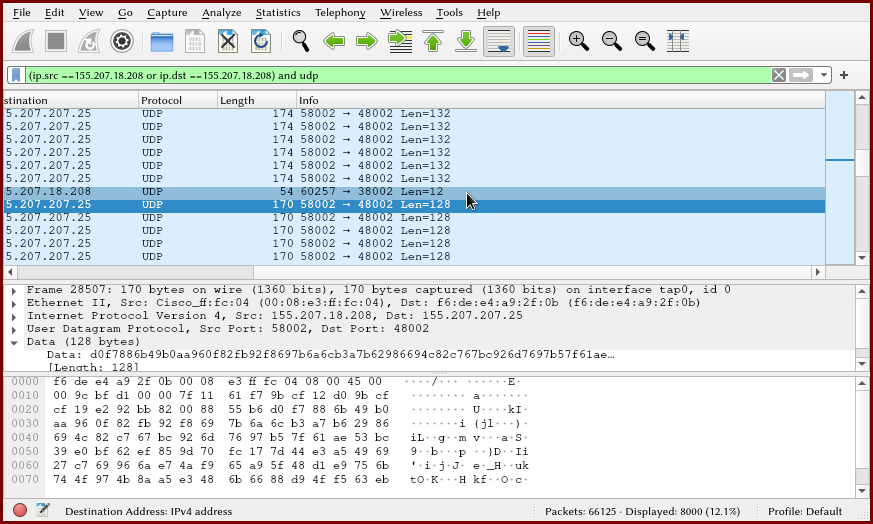
\includegraphics[width=\textwidth]{wireshark12.png}

\section{Ithaki Copter}
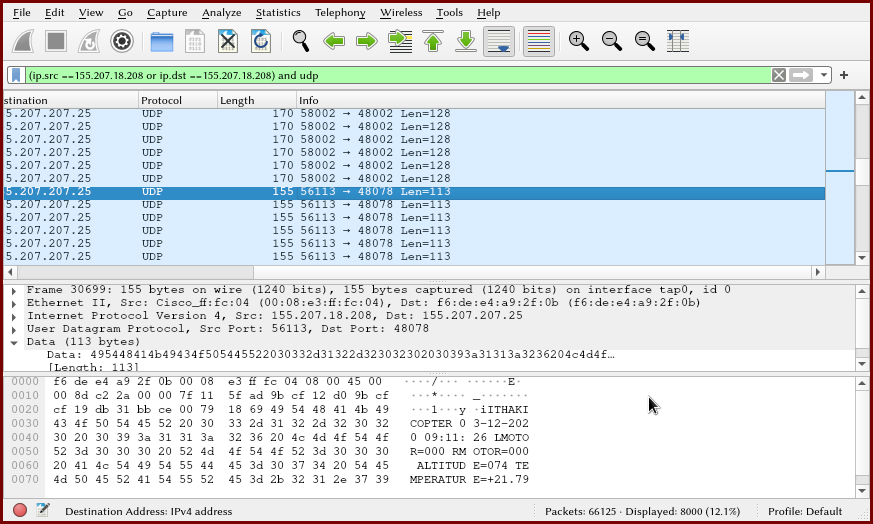
\includegraphics[width=\textwidth]{wireshark13.png}

\section{Vehicle}
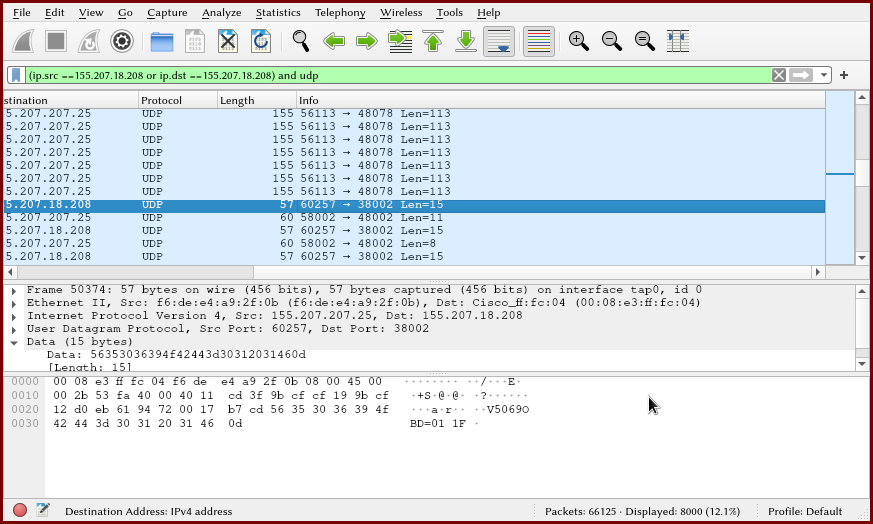
\includegraphics[width=\textwidth]{wireshark14.png}
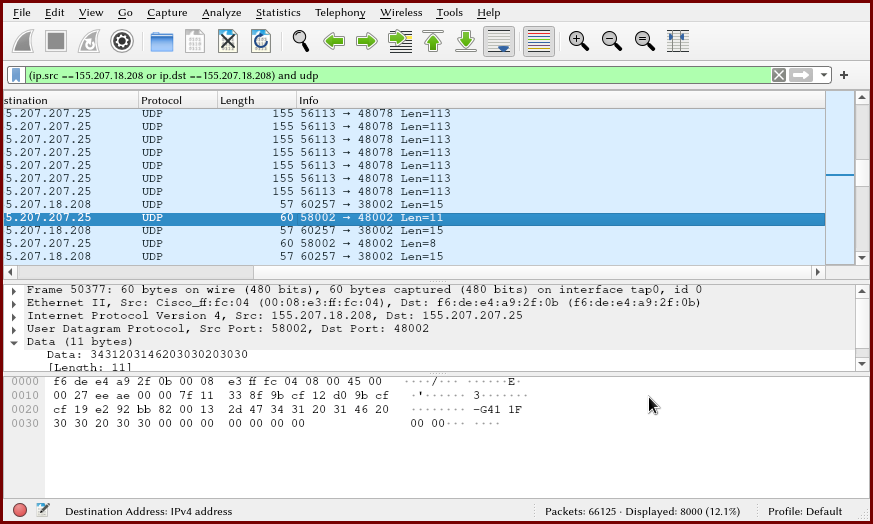
\includegraphics[width=\textwidth]{wireshark15.png}

\end{document}
